\documentclass{ML}
\usepackage{amsthm}
\usepackage{fontspec}
\usepackage[ruled,linesnumbered]{algorithm2e}

\setmonofont{Iosevka Nerd Font Mono}

\newtheorem{theorem}{定理}
% \newtheorem{proof}{证明}

% 姓名,学号
\infoauthor{冯云龙}{1160300202}

% 课程类型,实验名称
\infoexp{选修}{逻辑回归}

\begin{document}
\maketitle

\tableofcontents
\newpage

\section{实验目的}

\begin{enumerate}
	\item 理解逻辑回归模型
	\item 掌握逻辑回归模型的参数估计方法
	\item 实现两种损失函数的参数估计
	      \subitem 无惩罚项
	      \subitem 加入对参数的惩罚
	\item 掌握牛顿法
\end{enumerate}

\section{实验要求及实验环境}

\subsection{实验要求}

\begin{enumerate}
	\item 手工生成两个分别类别数据(使用高斯分布),验证算法
	\item 使用UCI数据集进行测试
\end{enumerate}

\subsection{实验环境}

\begin{itemize}
	\item 操作系统:Manjaro Linux x64
	\item 编程语言:Julia
	\item 绘图工具包:Plots.jl
	\item IDE:Atom (Juno)
\end{itemize}

\section{设计思想}

Logistic Regression虽然名字里带“回归”,但是它实际上是一种分类方法,用于两分类问题(即输出只有两种)。需要先找到一个预测函数(h),显然,该函数的输出必须是两个值(分别代表两个类别),所以利用了Logistic函数(或称为Sigmoid函数),函数形式为:

\begin{figure}[H]
	\centering
	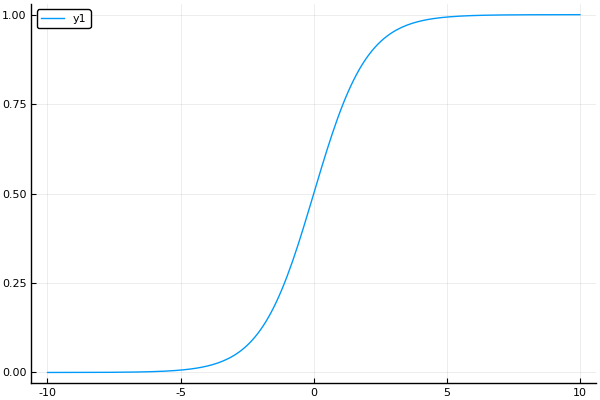
\includegraphics[width=0.36\linewidth]{media/sigmoid}
	\caption{$sigmoid(z) = \frac{1}{1 + e^{-z}}$}
	\label{fig:sigmoid}
\end{figure}

\subsection{算法原理}

\subsubsection{构造预测函数h(x)}

$$\begin{array}{ll}
		h_\theta(x) & = sigmoid(-\theta^TX)          \\
		            & = \frac{1}{1 + e^{-\theta^TX}}
	\end{array}$$

函数h(x)的值有特殊的含义,它表示结果取1的概率,因此对于输入x分类结果为类别1和类别0的概率分别为:

$$P(y=1│x;\theta)=h_\theta (x)$$
$$P(y=0│x;\theta)=1-h_\theta(x)$$

\subsubsection{构造损失函数}

由于我们知道y只能取0或者1,我们可以把概率写成如下形式:

$$P(y|x;\theta) = (h_\theta(x))^y(1-h_\theta(x))^{1-y}$$

取似然对数为:

$$L(\theta)=\prod_{i=1}^{m} {(h_{\theta}(x^{(i)}))^{y_i}} *{(1-h_{\theta}(x^{(i)}))^{1-y_i}}$$

取对数似然有:
$$l(\theta)=log(L(\theta))=\sum_{i=1}^{m}\log({(h_{\theta}(x^{(i)}))^{y_i}}) + \log({(1-h_{\theta}(x^{(i)}))^{1-y_i}})$$

$$l(\theta)=log(L(\theta))=\sum_{i=1}^{m} {y_i}log{(h_{\theta}(x^{(i)}))} + ({1-y_i})log{(1-h_{\theta}(x^{(i)}))}$$

我们的目标是使得l最大,即是

$$\theta = \arg \max_\theta l(\theta)$$

\subsection{算法的实现}

\subsubsection{梯度下降}

求导:


$$\begin{array}{ll}
		\frac{\partial l}{\partial \theta_j} & =  ∑^m_{i=1}(y_i \frac{1}{h_\theta(x^{(i)})} \frac{\partial h_\theta}{\partial \theta_j} -(1-y_i)\frac{1}{1-h_\theta(x^{(i)})}\frac{\partial h_\theta}{\partial \theta_j}) \\
		                                     & = ∑^m_{i=1}(y_i \frac{1}{g(\theta^Tx^{(i)})} - (1-y_i)\frac{1}{1 - g(\theta^Tx^{(i)})})\frac{\partial g(\theta^Tx^{(i)})}{\partial \theta_j}                               \\
		                                     & = ∑^m_{i=1}(y_i \frac{1}{g(\theta^Tx^{(i)})} - (1-y_i)\frac{1}{1 - g(\theta^Tx^{(i)})})g(\theta^Tx^{(i)})(1-g(\theta^Tx^{(i)}))\frac{\theta^Tx^{(i)}}{\partial \theta
		_j}                                                                                                                                                                                                               \\
		                                     & = ∑^m_{i=1}(y_i(1-g(\theta^Tx^{(i)})) - (1-y_i)g(\theta^Tx^{(i)}))x^{(i)}_j                                                                                                \\
		                                     & = ∑^m_{i=1}(y_i-g(\theta^Tx^{(i)}))x^{(i)}_j                                                                                                                               \\
		                                     & = ∑^m_{i=1}(y_i - h_\theta(x^{(i)}))x^{(i)}_j
	\end{array}$$

$$\theta_j = \theta_j - α \frac{1}{m}∑^m_{i=1}(h_\theta(x^{(i)})-y_i)x^{(i)}_j$$

向量化之后我们有:

$$X = \begin{bmatrix}
		x^{(1)} \\
		⋮       \\
		x^{(m)}
	\end{bmatrix} = \begin{bmatrix}
		x_{11} & \dots & x_{1n} \\
		⋮      &       & ⋮      \\
		x_{m1} & \dots & x_{mn}
	\end{bmatrix}
	Y = \begin{bmatrix}
		y_1 \\
		⋮   \\
		y_m
	\end{bmatrix}
	θ = \begin{bmatrix}
		θ_1 \\
		⋮   \\
		θ_n
	\end{bmatrix}$$

$$\hat{Y} = X θ = \begin{bmatrix}
		x_{11} & \dots & x_{1n} \\
		⋮      &       & ⋮      \\
		x_{m1} & \dots & x_{mn}
	\end{bmatrix} \begin{bmatrix}
		θ_1 \\
		⋮   \\
		θ_n
	\end{bmatrix} = \begin{bmatrix}
		θ_1x_{11} & \dots & θ_nx_{1n} \\
		⋮         &       & ⋮         \\
		θ_1x_{m1} & \dots & θ_nx_{mn}
	\end{bmatrix}
$$

$$E = h_θ(X) - Y = \begin{bmatrix}
		h_θ(x^{(1)})-y_1 \\
		⋮                \\
		h_θ(x^{(m)}) - y_m
	\end{bmatrix}$$

$$θ = θ - αX^TE$$

\subsubsection{牛顿法}

考虑牛顿法在求解方程$f(\theta)=0$时的用法。牛顿法在求解方程根时,主要是根据泰勒展示式进行迭代求解的。 假设 $f(x)=0$ 有近似根$x_k$,那么 $f(x)$ 在点 $x_k$ 处的泰勒展开式表示为,

$$f(x) \approx f(x_k) + f'(x_k)(x-x_k)$$

令$f(x)=0$有,$f(x_k)+f′(x_k)(x−x_k)=0$,求解得到$x_{k+1}$

$$x_{k+1}=x_{k}-\frac{f(x_k)}{f'(x_k)}$$

类似的,我们求解$\theta$

$$\theta = \theta - \frac{l'(\theta)}{l''(\theta)}$$

$$\frac{\partial }{\partial\theta_i}l(\theta)=\sum_{t=1}^m(y^{(t)}-h_\theta(x^{(t)}))x_i^{(t)}$$

$$\begin{array}{ll}
		H_{ij}
		 & =\frac{\partial^2l(\theta)}{\partial \theta_i\partial \theta_j}                                               \\
		 & =\frac{\partial }{\theta_j}\sum_{t=1}^m(y^{(t)}-h_\theta(x^{(t)}))x_i^{(t)}                                   \\
		 & =\sum_{t=1}^m \frac{\partial }{\theta_j} (y^{(t)}-h_\theta(x^{(t)}))x_i^{(t)}                                 \\
		 & =\sum_{t=1}^m -x_i^{(t)} \frac{\partial}{\partial\theta_j}h_\theta(x^{(t)})                                   \\
		 & =\sum_{t=1}^m -x_i^{(t)} h_\theta(x^{(i)}) (1-h_\theta(x^{(i)})) \frac{\partial }{\theta_j}(\theta^Tx^{(t)} ) \\
		 & =\sum_{t=1}^m h_\theta(x^{(t)})(h_\theta(x^{(t)})-1)x^{(t)}_ix^{(t)}_j                                        \\
	\end{array}$$

$$A=\begin{bmatrix}
		h_θ(x^{(1)})\cdot [h_θ(x^{(1)})-1] & 0                                  & \cdots & 0                                  \\
		0                                  & h_θ(x^{(2)})\cdot [h_θ(x^{(2)})-1] & \cdots & 0                                  \\
		\vdots                             & \vdots                             & \ddots & \vdots                             \\
		0                                  & 0                                  & \cdots & h_θ(x^{(m)})\cdot [h_θ(x^{(m)})-1] \\
	\end{bmatrix}$$

$$U = - X^T E=  \begin{bmatrix}
		x_{11} & x_{21} & \cdots & x_{m1} \\
		x_{12} & x_{22} & \cdots & x_{m2} \\
		\vdots & \vdots & \ddots & \vdots \\
		x_{1n} & x_{2n} & \cdots & x_{mn}
	\end{bmatrix}
	\begin{bmatrix}
		y_1 - h_θ(x^{(1)}) \\
		y_2 - h_θ(x^{(2)}) \\
		\vdots             \\
		y_m - h_θ(x^{(m)}) \\
	\end{bmatrix}$$

$$H = X^T A X$$

$$θ_{new}=θ_{old}-\frac{U}{H}=θ_{old}-{H}^{-1}{U}$$

\section{实验结果与分析}

\begin{figure}[H]
	\begin{minipage}[c]{0.5\linewidth}
		\centering
		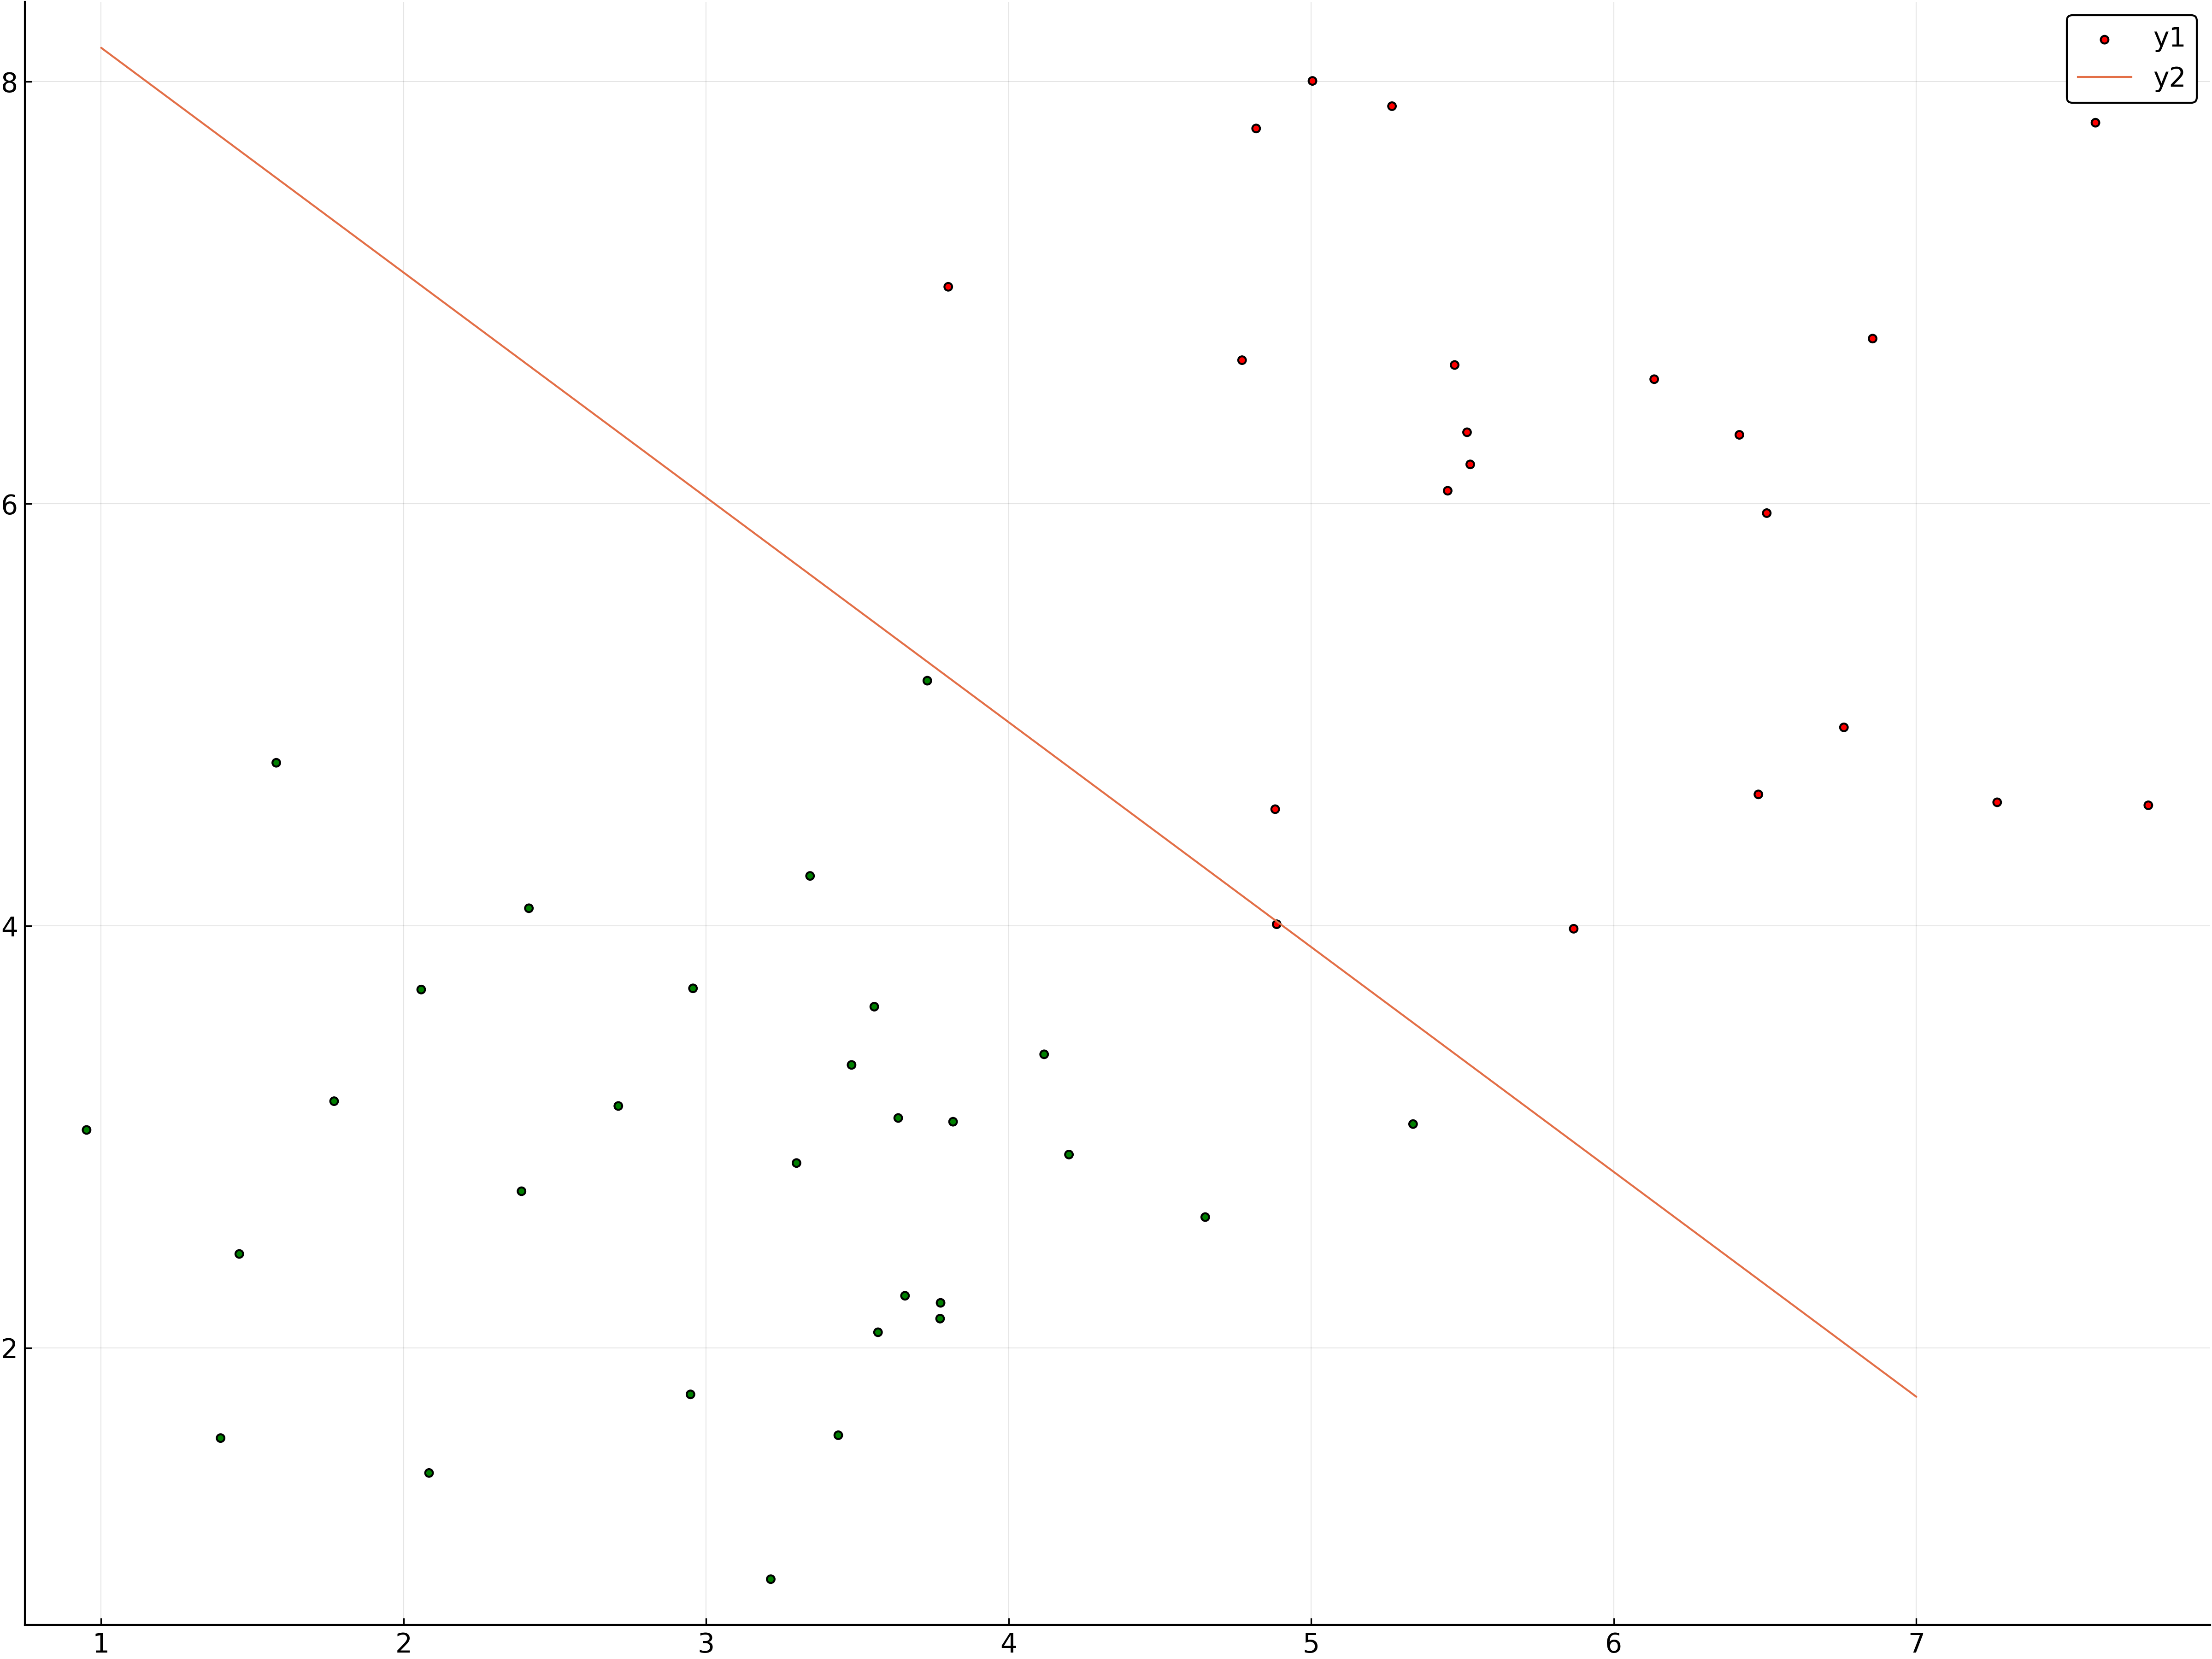
\includegraphics[width=0.9\linewidth]{media/Logistic/grad-plot}
		\caption{梯度下降法决策面}
		\label{fig:grad-plot}
	\end{minipage}
	\begin{minipage}[c]{0.5\linewidth}
		\centering
		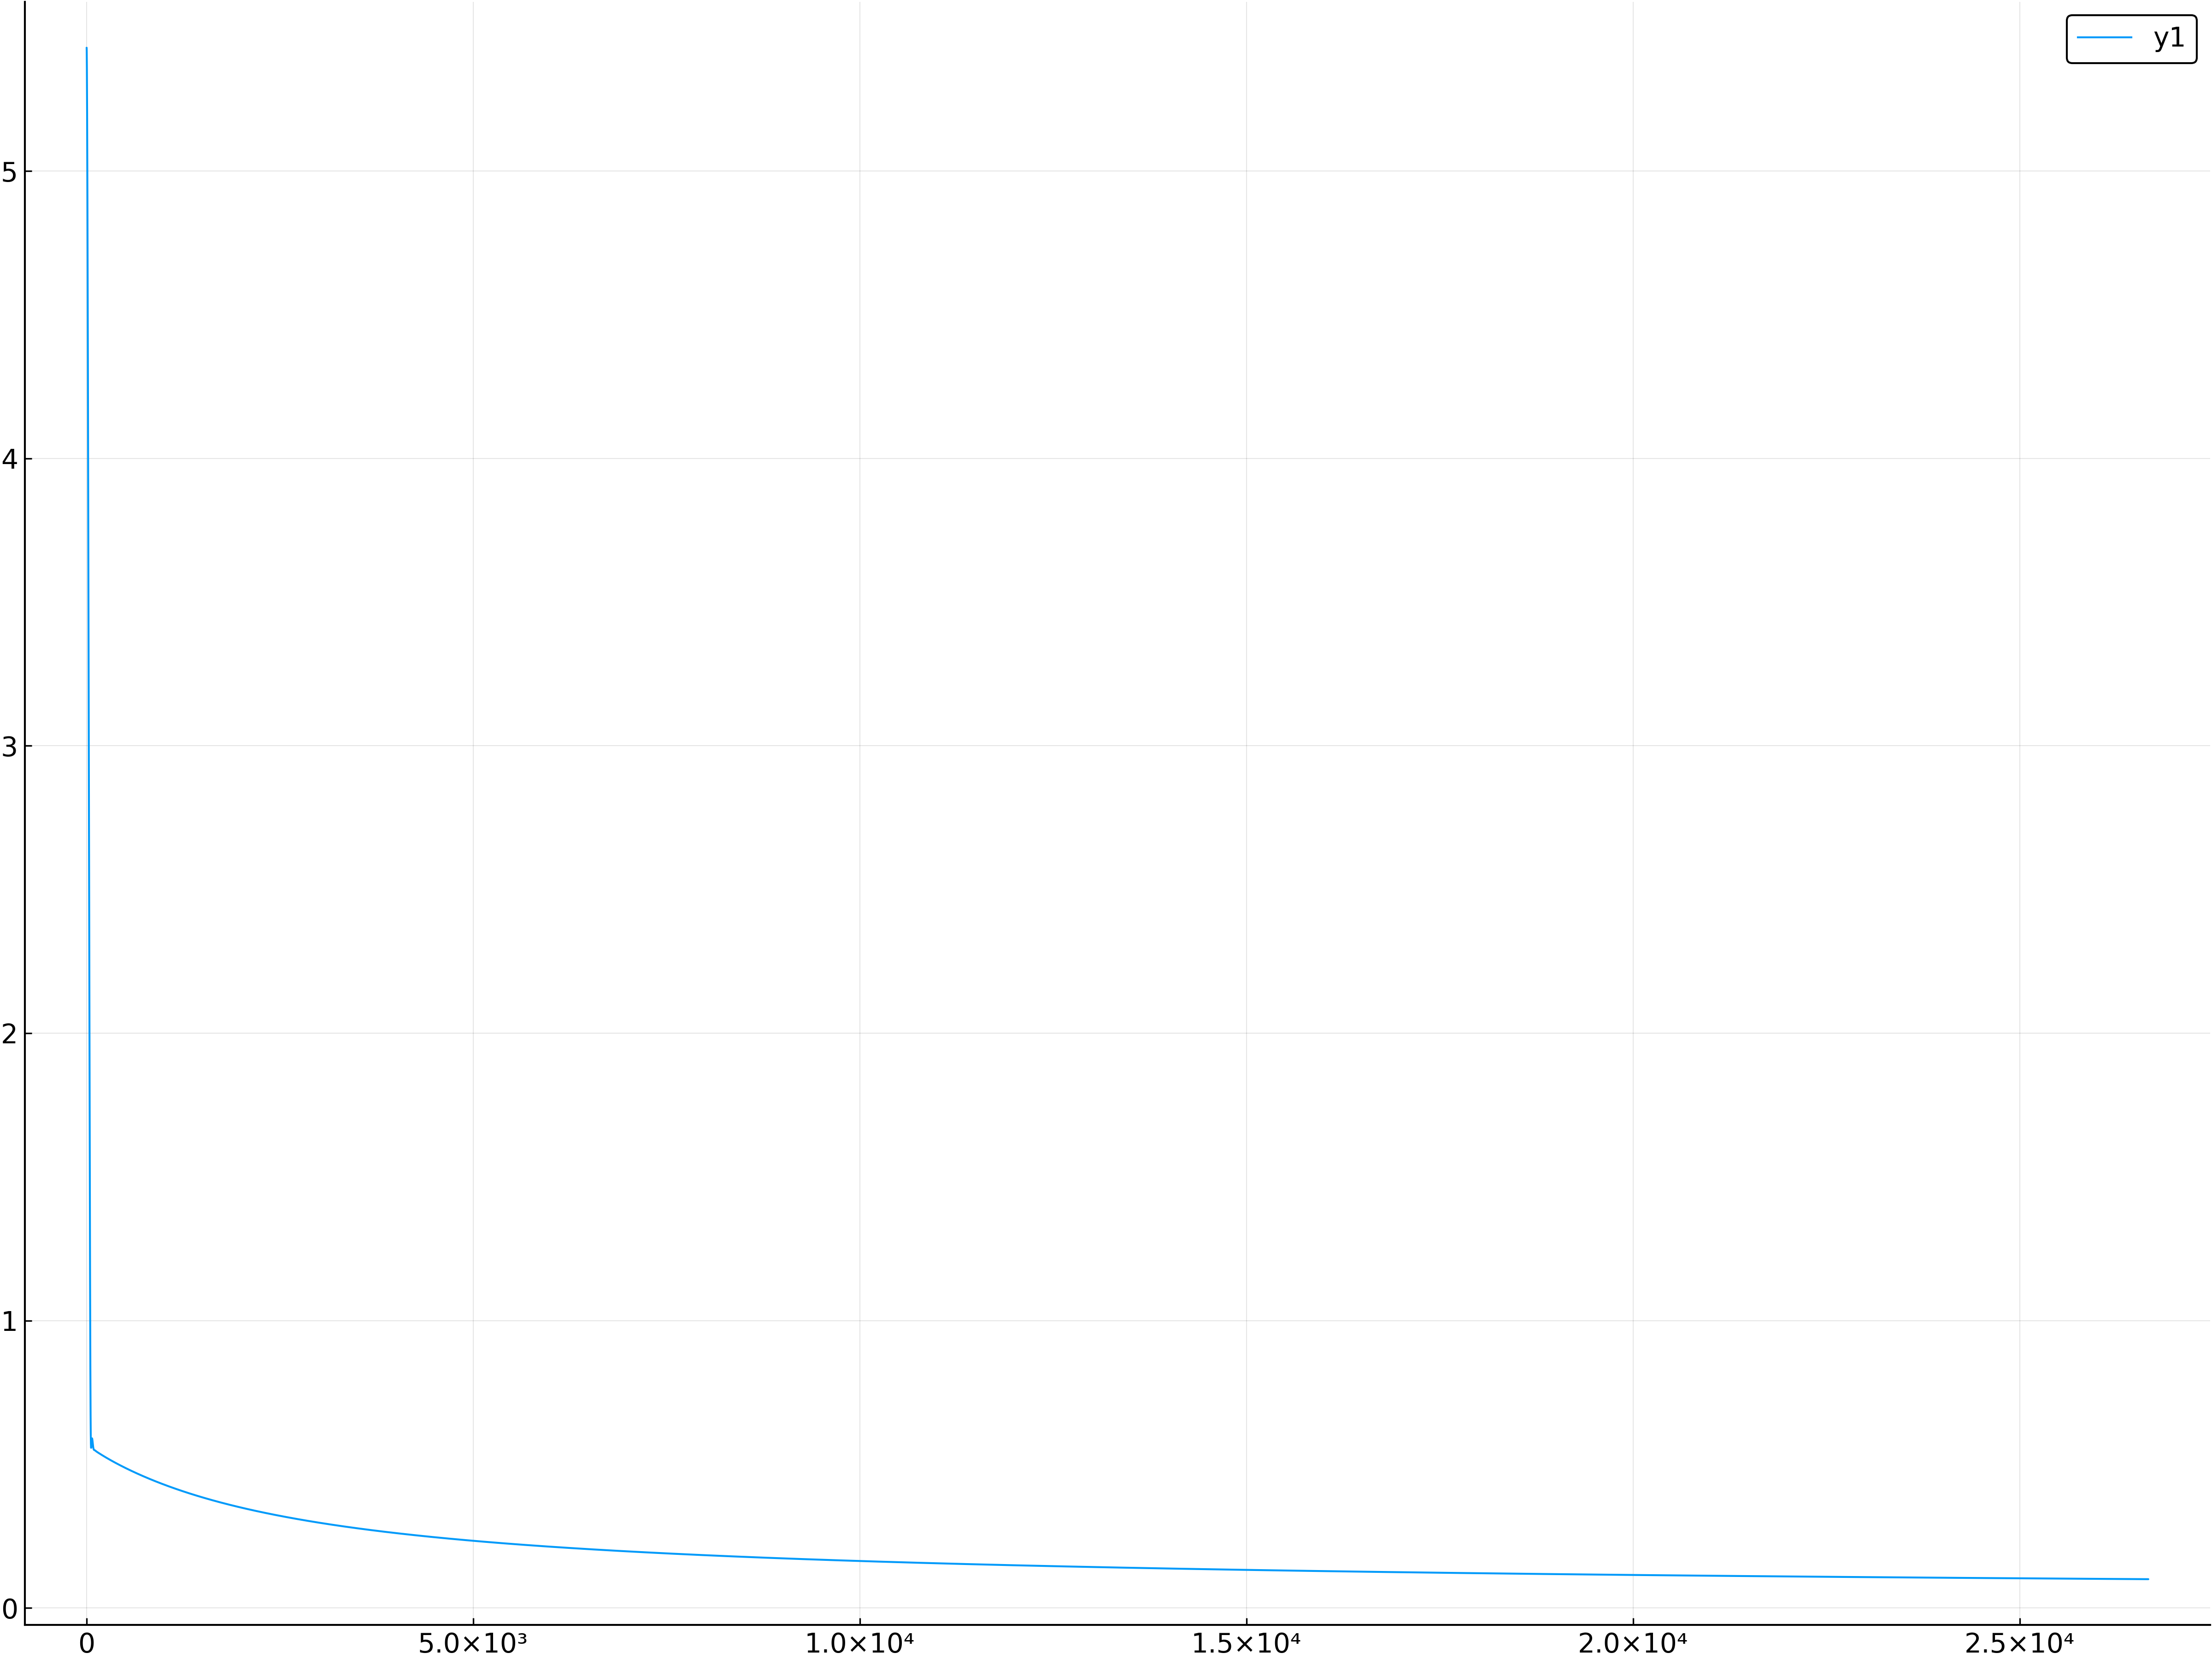
\includegraphics[width=0.9\linewidth]{media/Logistic/grad-loss}
		\caption{梯度下降法损失}
		\label{fig:grad-loss}
	\end{minipage}
\end{figure}

\begin{figure}[H]
	\begin{minipage}[c]{0.5\linewidth}
		\centering
		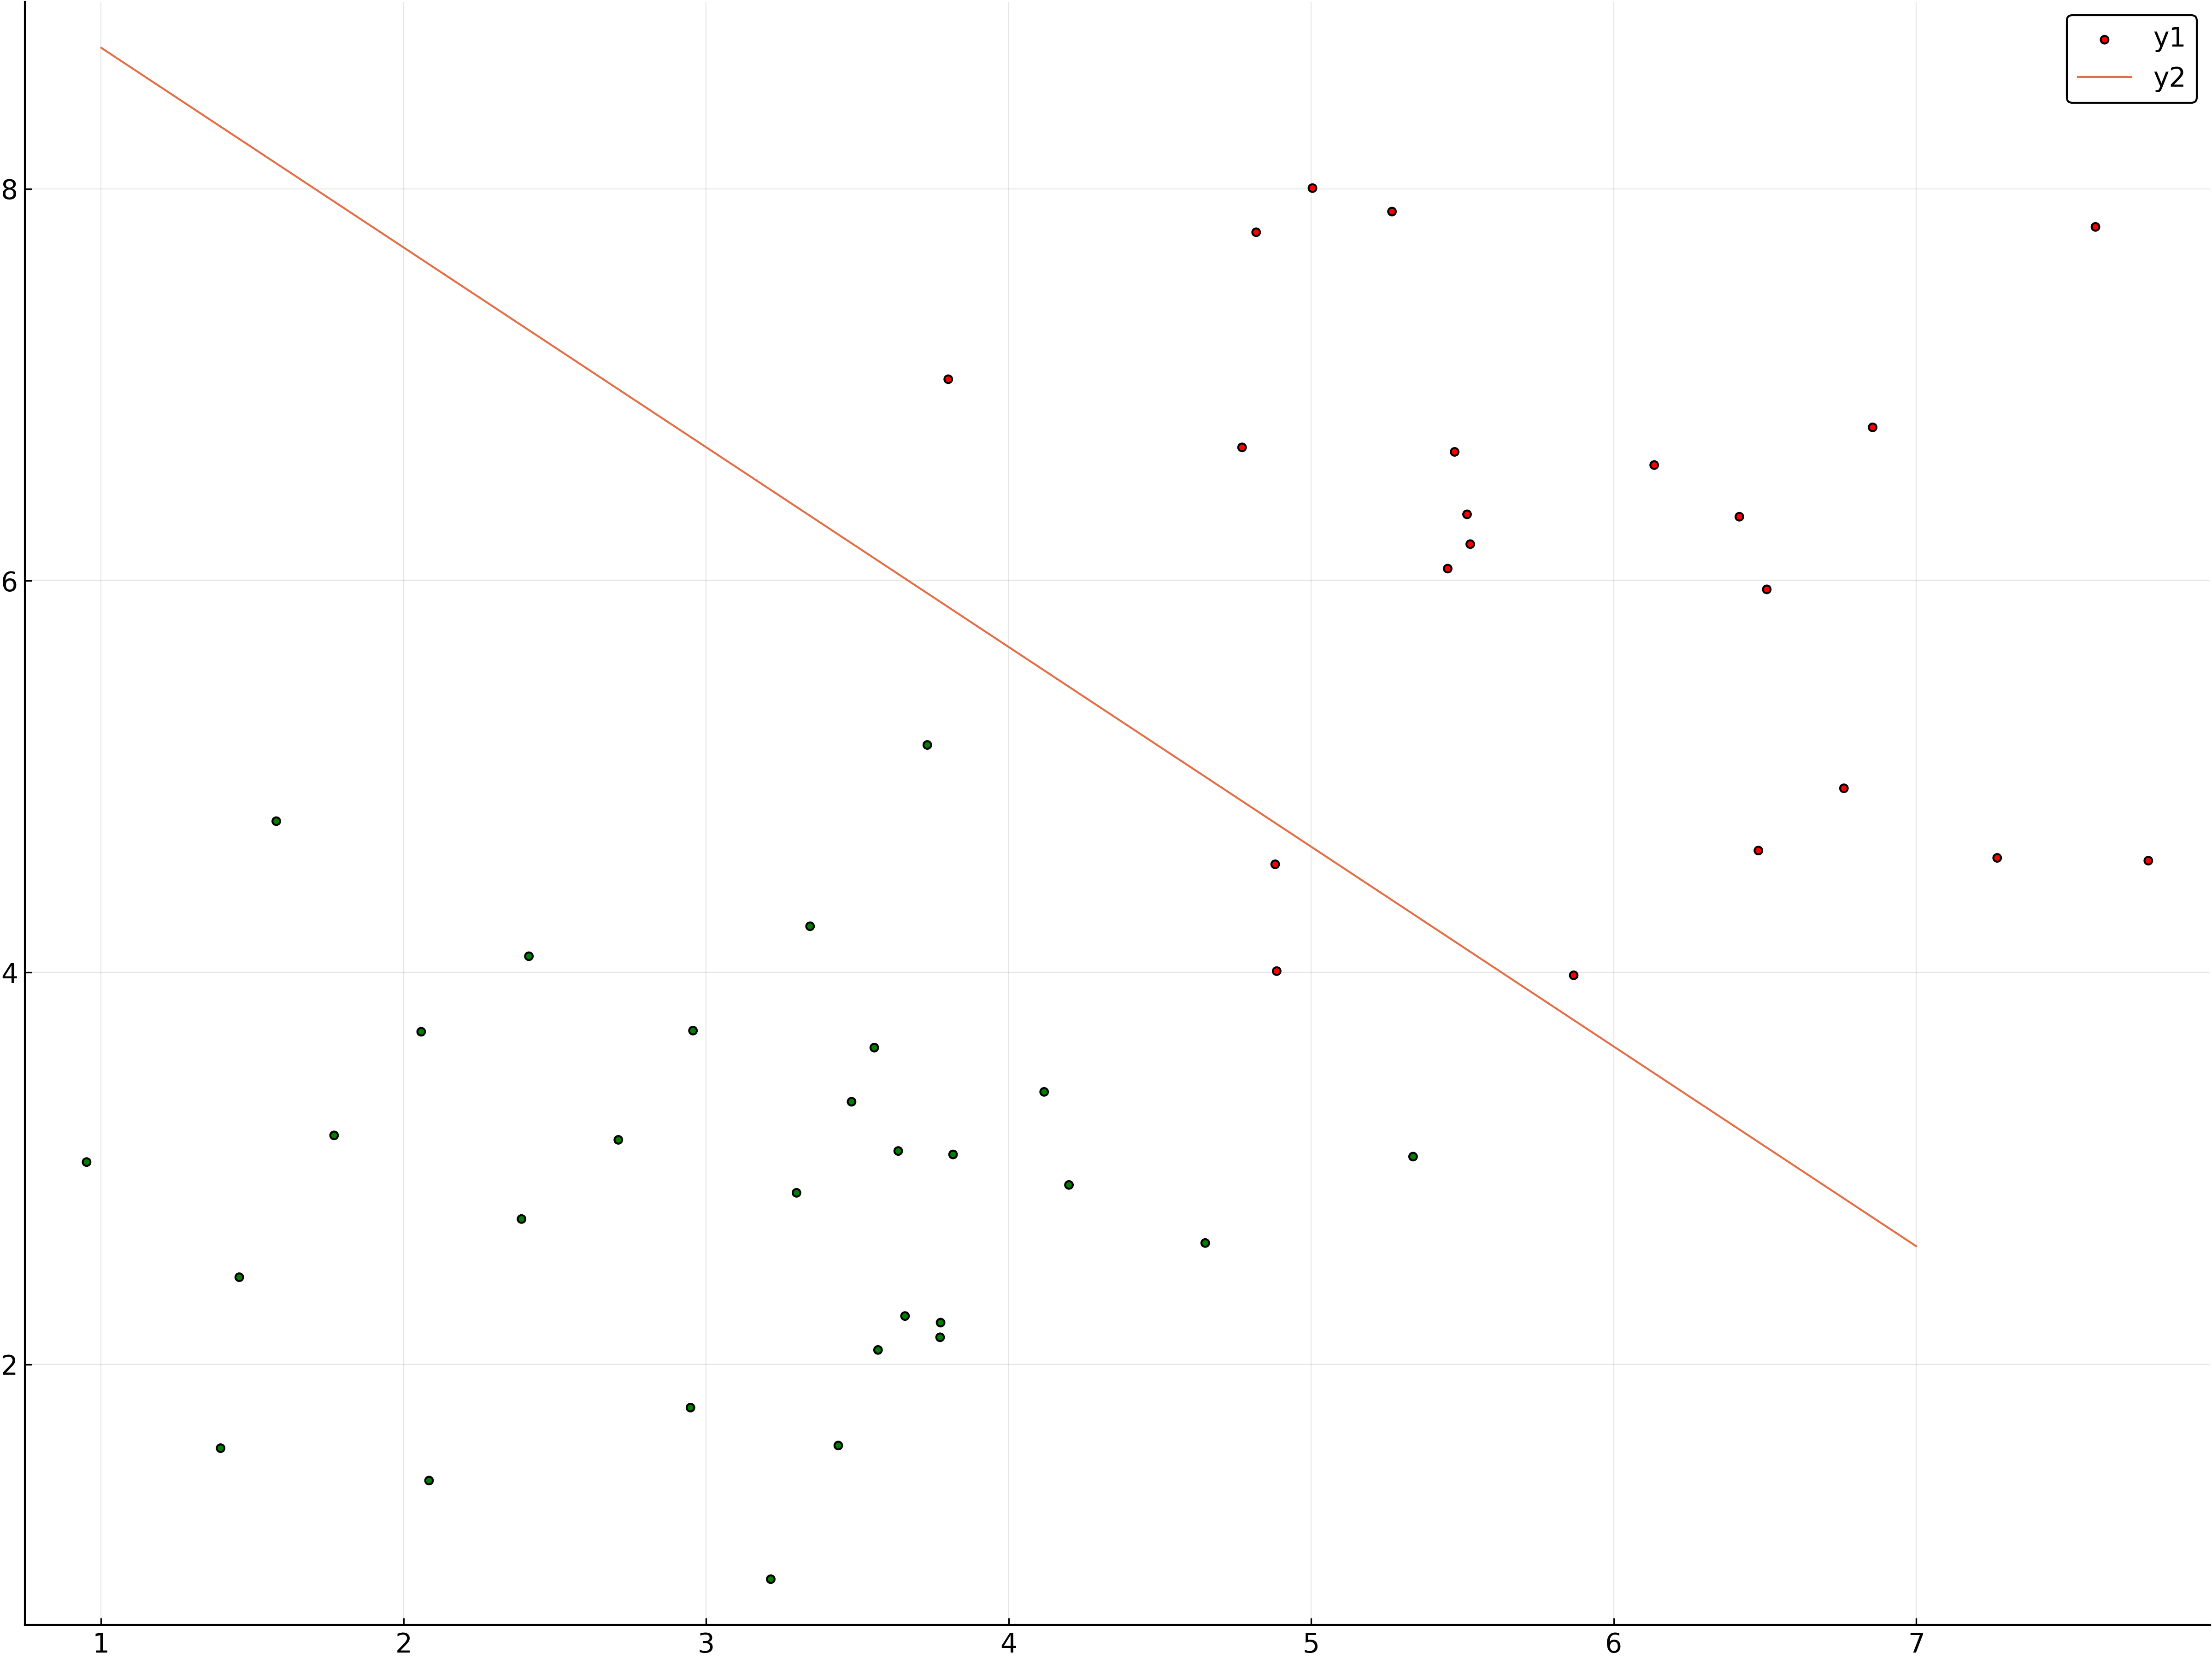
\includegraphics[width=0.9\linewidth]{media/Logistic/newtown-plot}
		\caption{牛顿法决策面}
		\label{fig:newtown-plot}
	\end{minipage}
	\begin{minipage}[c]{0.5\linewidth}
		\centering
		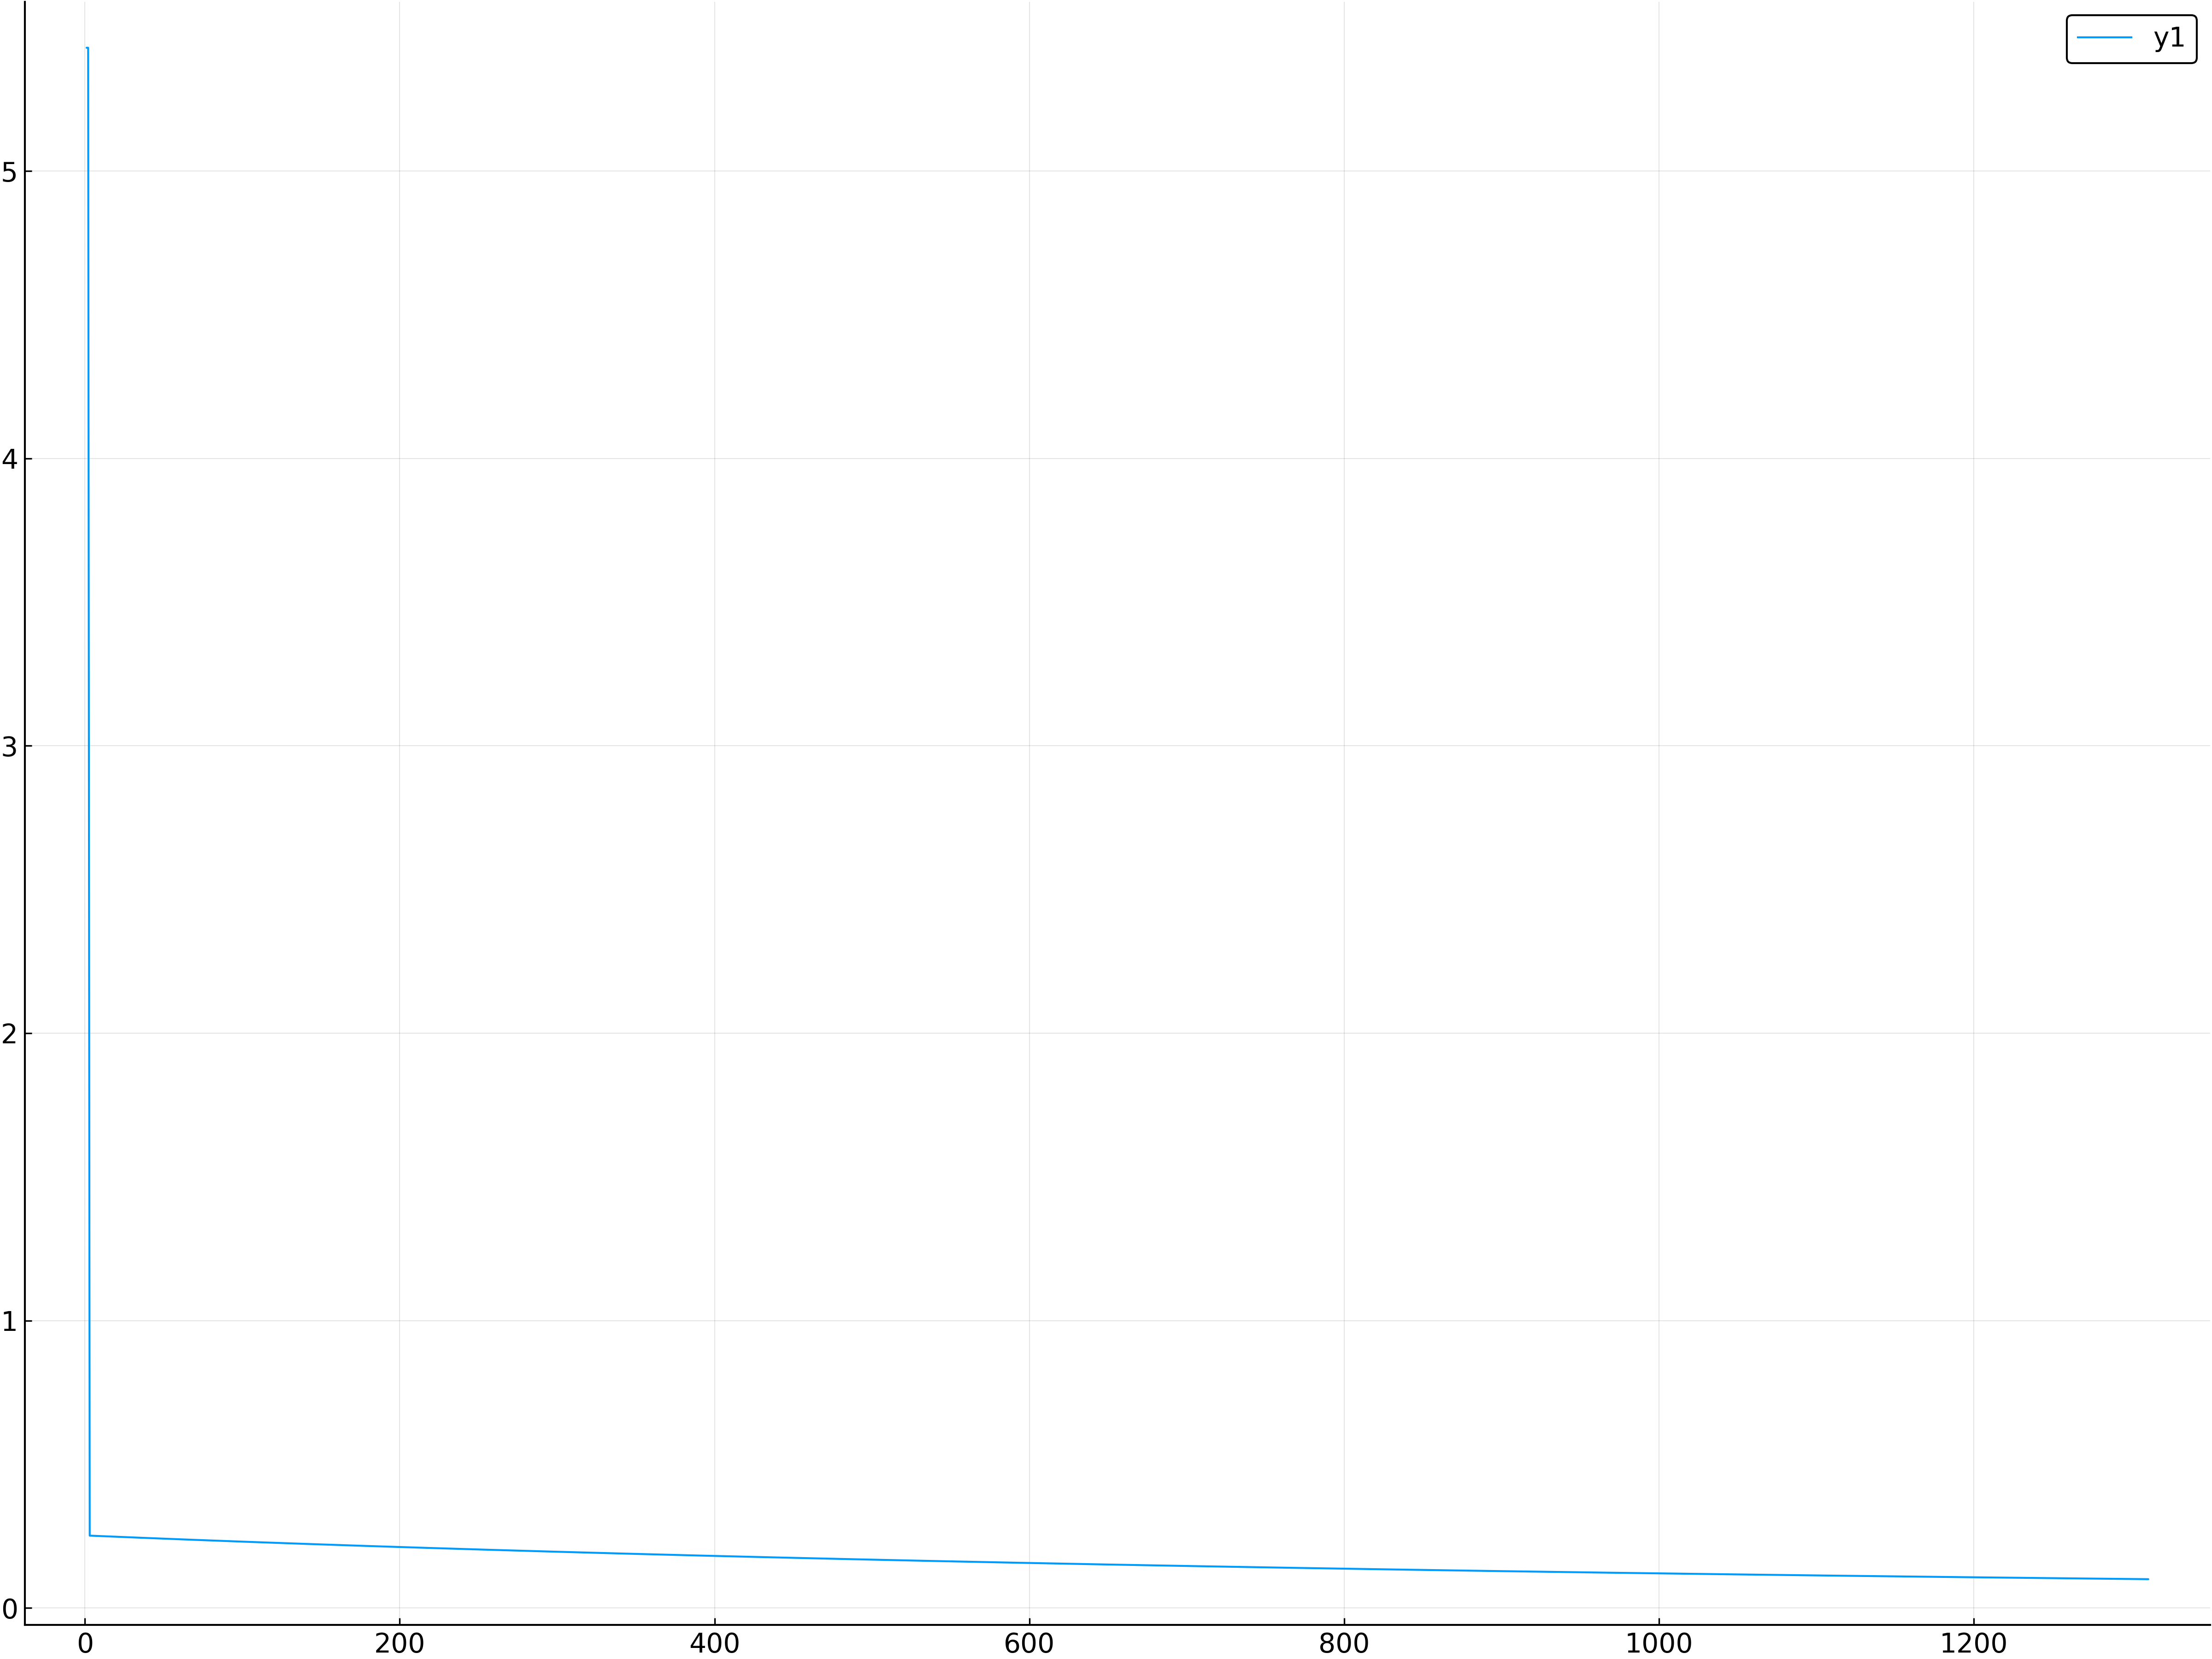
\includegraphics[width=0.9\linewidth]{media/Logistic/newtown-loss}
		\caption{牛顿法损失,可以看到这里下降到0.1以下只迭代了1300轮不到,相比梯度下降法的260000轮,相差的量级巨大}
		\label{fig:newtown-loss}
	\end{minipage}
\end{figure}

在本次实验中加入正则项和不加入正则项,差异不大,代码中已经实现,这里不再展示,牛顿法使用二阶导数,下降的速率是相当快速的。

之后我使用了UCI的鸢尾花数据集进行测试,由于是多个维度的数据,我这里就仅绘制loss。

\begin{figure}[H]
	\centering
	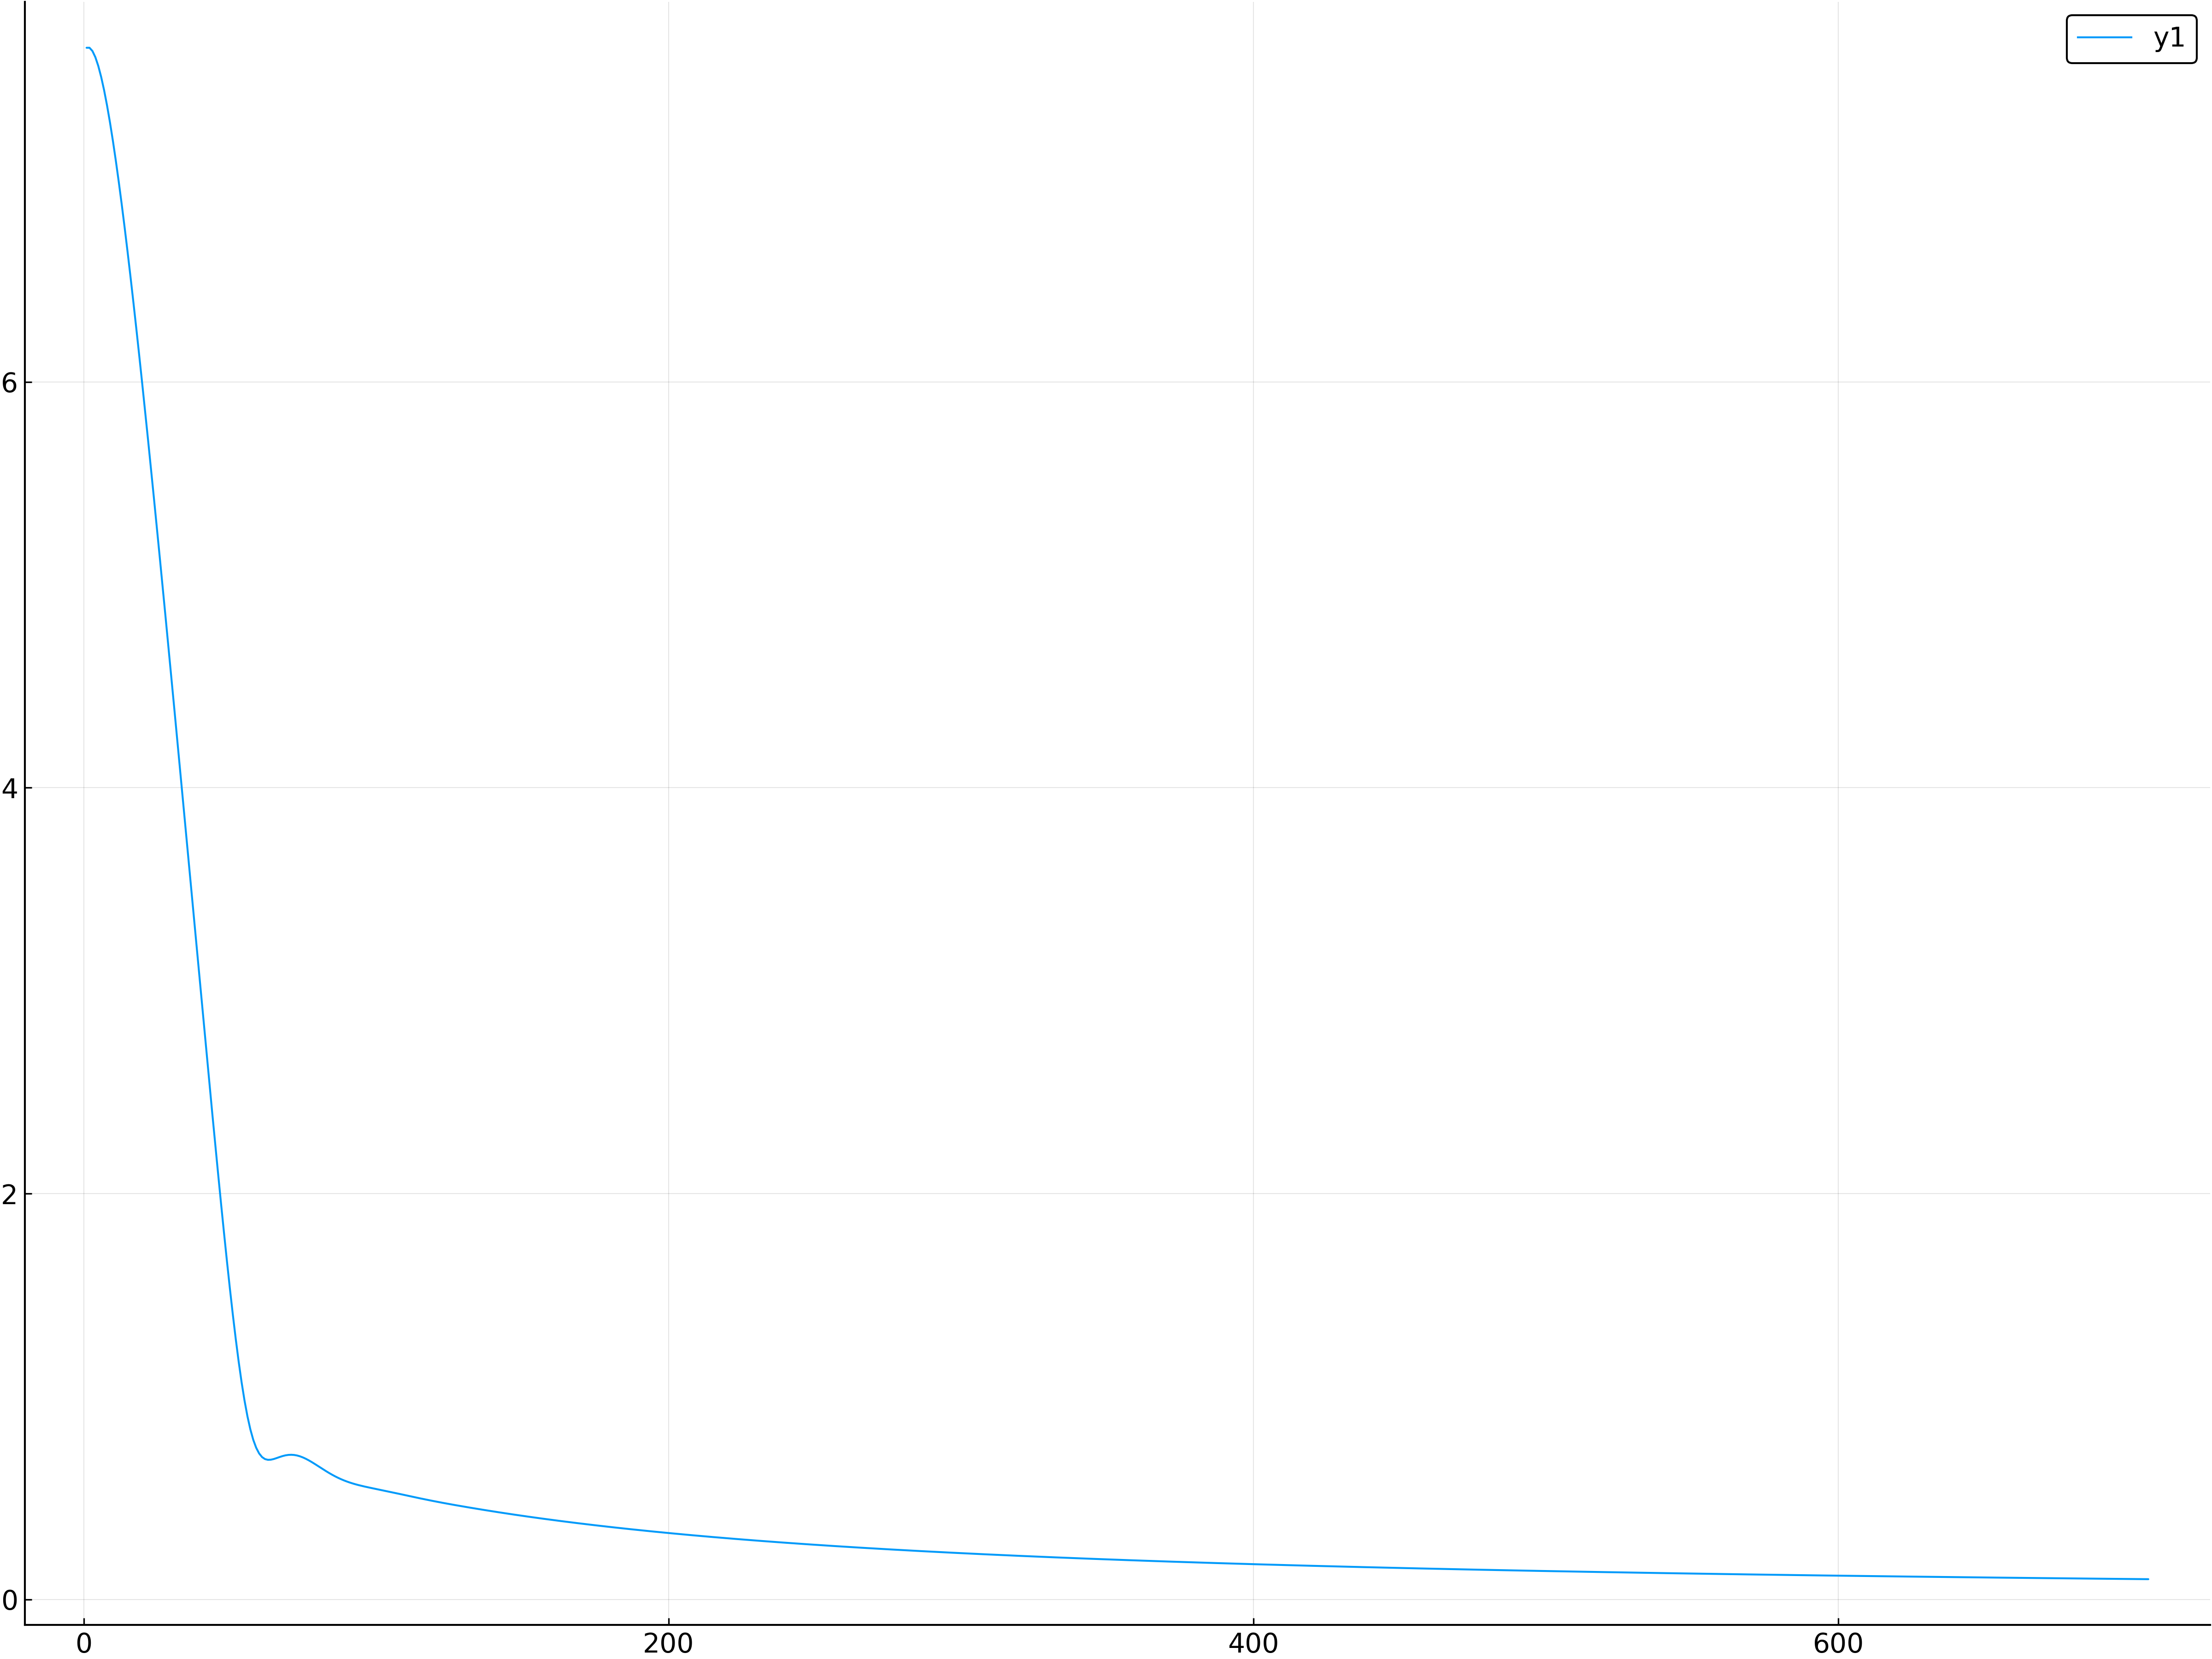
\includegraphics[width=0.9\linewidth]{media/Logistic/iris-loss}
	\caption{鸢尾花数据集}
	\label{fig:iris-loss}
\end{figure}

\section{结论}

这里总结一下逻辑回归的优缺点:

\paragraph{优点:}
\begin{enumerate}
\item 速度快,适合二分类问题
\item 简单易于理解,直接看到各个特征的权重
\item 能容易地更新模型吸收新的数据
\end{enumerate}


\paragraph{缺点:}
对数据和场景的适应能力有局限性,不如决策树算法适应性那么强

\appendix

\section{源代码}

\inputminted[breaklines=true,frame=lines,mathescape=true]{julia}{../LogisticRegression.jl}

\end{document}
